\documentclass[11pt]{IEEEtran}
% Packages
\usepackage{graphicx}
\usepackage{amsmath} 
\usepackage{mathtools}
\usepackage{epstopdf}
\usepackage{float}
\usepackage{textcomp}
\usepackage{amssymb}
\usepackage{cite}
\usepackage[dvipsnames]{xcolor}
\usepackage{listings}
\lstset{%
  basicstyle=\ttfamily,
  breaklines=true,
  columns=fullflexible,
  frame=single,
  frameround=tttt,
  showstringspaces=false,
}

% Title stuff
\title{Classification of Web Advertisements}

\author{Sameer Chauhan, Michael Scibor, Christian Sherland\\
\texttt{chauha3@cooper.edu, scibor@cooper.edu , sherla@cooper.edu}\\
Department of Electrical Engineering\\
The Cooper Union\\
41 Cooper Square\\
New York, NY 10003
\thanks{ Thanks Professor Sam Keene}}

% Journal Info
\markboth{Journal of Makeene Learning, ̃Vol . ̃1, No. ̃1, ̃Dec ̃2013}{Shell \MakeLowercase{\text it{et al.}}: A Novel Tin Can Link}
\IEEEpubid{2718--2818/00\$50.00 ̃\copyright ̃2013 IEEE }

\begin{document}
\maketitle

\begin{abstract}
Advertisements can be very intrusive on the internet in many places and so their have been many attempts to block internet ads. This paper explores the characterization of internet advertisements from HTML metadata. Specifically, we explore machine learning techniques such as k-nearest neighbors and tree bagger to classify images on webpages as ad or non ads. This paper also explores a possible minimal set of features for accurate classification of internet advertisements.
\end{abstract}

\begin{IEEEkeywords}
TreeBagger, KNN, PRT, Machine Learning, Feature Selection
\end{IEEEkeywords}

\section{Introduction}
Advertisements are on of the driving forces behind free content on the internet. However, they are often intrusive and unwanted, and their increased prevalence on the internet has resulted in aggravation for many users. This has led to the development of various techniques for blocking internet advertisements. 

Most current methods for blocking advertisements on the internet use black lists or white lists: these are lists of either forbidden or accepted content that are cross referenced with the content of a webpage through the use of regular expressions to determine what should be marked as an advertisement and blocked from the user. 

This method works well for most content, however, the major issue is that it requires maintaining an up-to-date blacklist, but with new websites surfacing every second, this becomes a tedious effort.  If an advertisement is not contained within the blacklist, that advertisement will not be blocked. As such, this approach works very well for data described in a black list, but fails entirely for all other data.

This motivates the question - can we create an advertisement blocking system that does not utilize a black list? It seems that many advertisements on the internet share certain features, and therefore it may be possible to determine patterns that can be used to classify content on the internet as either being an advertisement or not.

The remainder of this paper explores existing approaches, various machine learning techniques for this problem, possible features that perform well for this type of classification problem and proposes a method for blocking internet advertisements. Additionally, further improvements to the system that we implemented are discussed.

\section{Prior Work}
The most popular advertisement blocking system today is an internet browser plugin called AdBlock Plus. AdBlock Plus works by cross checking internet content with filter lists which tell it if content is an advertisement or not. Any content that it determines to be an advertisement is not displayed to the user\cite{adblock}. Essentially this is how blacklist systems work and is how many existing systems are implemented.

\begin{figure}[h!]
  \caption{AdEater Architecture}
  \label{adeaterimg}
  \centering
    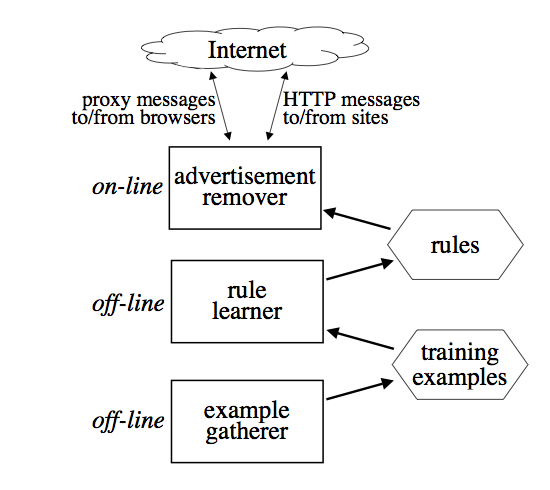
\includegraphics[width=0.5\textwidth]{Figures/adeater.png}
\end{figure}

An advertisement blocking system that functioned using machine learning techniques was previously explored by Nicholas Kushmeric with the development of AdEater. \cite{adeater}. Figure  1 shows how data flows through the AdEater system in order to classify internet advertisements. The AdEater trains its machine learning algorithm offline using a 1558 feature dataset which is generated by scrapping the web. The data is now hosted on the UCI Data Repository website\cite{uci} and contains features about the following advertisement properties:
\begin{itemize}
\item Image Geometry
\item URL
\item Text
\end{itemize}
The image geometry features describe the height, width and aspect ratio of the image which is useful for targeting banner and sidebar ads. The URL features relate the URL of the website with the URL of the image and the website to which the image is linking. The URL features were used to determine if the image was hosted outside of the host website or if the image linked to a website  The majority of the features were generated from related text as they contain information about the alt text, caption, and other surrounding words.  

Kushmeric's goal was to train a C4.5 rules learning algorithm offline and allow for almost  instant classification within a web browser. Implementing the algorithm this way allows for a longer training period if the classification time is significantly less. The C4.5 algorithm is a statistical classifier which generates a decision tree that links relavent features to a set of learned rules for an advertisement. Even though this simple algorithm achieved $97.2\%$ accuracy, we believe that acceptable results could be attained with a smaller feature space and that the system could benefit from a more powerful classifier.



\section{Classification}
\IEEEpubidadjcol
Our initial approach to this problem was to test a variety of distinct classifiers in an effort to improve upon the amount of properly classified elements and determine what classifier would be best to proceed with.

\begin{figure}[h!]
  	\label{compall}
  	\centering
    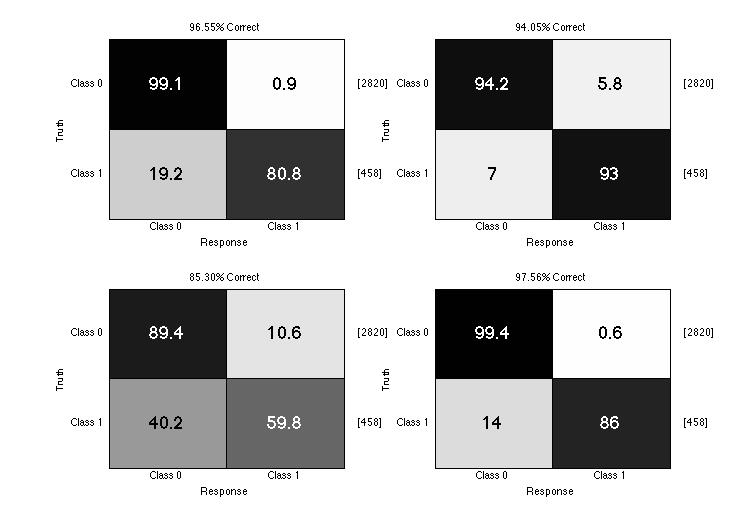
\includegraphics[width=0.5\textwidth]{Figures/allcomp.jpg}
	\caption{Confusion Matrices for KNN (top left), SVM (top right), RVM (bottom left) and Tree Bagger (bottom right)}
\end{figure}

We attempted to classify this data using a Support Vector Machine (SVM), Relevance Vector Machine (RVM), K-Nearest Neighbours, and a Tree Bagger. When choosing these algorithms, it is important to remember that a long training phase is acceptable, as long as the desired algorithm has a quick classification time. The performance of these classifiers was determined using k-folds on our training data with 10 folds. The results of this test are shown in Figures 2.

The results in Figure 1 are displayed as confusion matrices describing the correct classification and misclassification of each classifier. As can be seen the TreeBagger performs the best with about 98\% correct classification in 10 folds. This value is more or less consistent with the results achieved in \cite{adeater}. We were not able to exceed the results of \cite{adeater}. 

The RVM was clearly the worst performing of the algorithms and so we immediately eliminated that as a choice for classifier. It seemed that misclassification of legitimate content was worse than misclassification of advertisements, so we valued very highly the percent of non-ads classified. As such, because of its performance the Tree Bagger became the clear choice for continued work. 

It is also worth noting that there is an inherent bias within the data. There are approximately 2500 examples of advertisements and 500 examples of non-advertisements. We chose to work with all examples for training so that we could make comparisons \cite{adeater}. However, it is possible that this may skew the results slightly.

\section{Feature Space Reduction}
While the TreeBagger classifier performed well on this dataset, there were over 1,000 features to consider, and we were curious to see if it was possible to get similar results with only a small subset of the feature space. There are two major benefits to this:

\begin{enumerate}
\item The classifier would be trained faster. 
\item The amount of information necessary to properly classify an element would be reduced.
\end{enumerate}

If this system with a reduced feature set were implemented as a browser plug-in, this would mean faster page load times and consequently, a better user experience. 

Additionally, we felt that much of the feature data imitated what is usually done in white lists and black lists: for example, some of the features in the dataset are the source urls for images. We wanted to avoid using black lists as a reference for classification, and decided that a smaller subset of the feature space which does not consider these features was a more sincere machine learning approach to this problem.

In order to determine which features would be most useful for classification of advertisements, we first decided to look at the correlation between each of the individual features and the output\cite{feat}. The idea was that features more strongly correlated with the output are the features that are more useful for classification. The results of our feature selection choices are shown in Figure 3.

\begin{figure}[h!]
  	\label{featselall}
  	\centering
    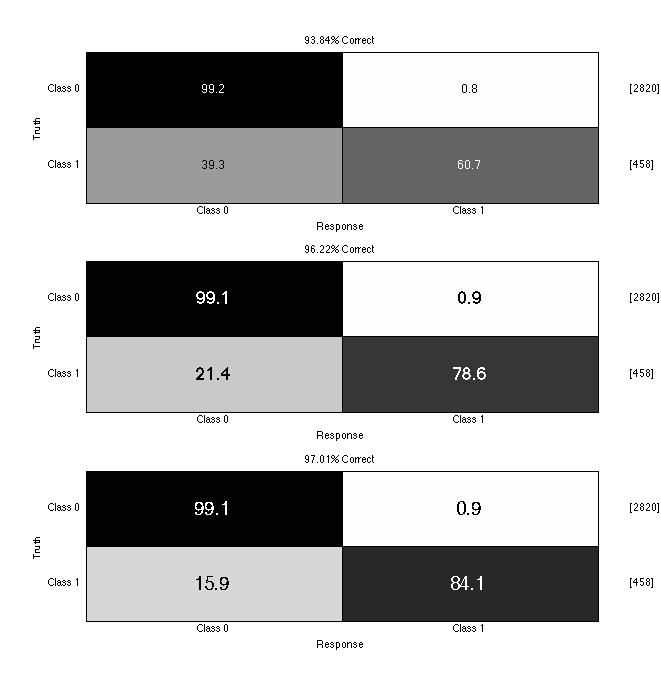
\includegraphics[width=0.5\textwidth]{Figures/featselall.jpg}
	\caption{Confusion Matrices for Selection by Entropy (Top), Selection by Correlation with Output (Middle) and Selection by PRT (Bottom)}
\end{figure}
 
We found that this subset of features achieved high correct classification with a significant reduction in the dimensionality of the feature space. It was apparent that much of the feature data was extraneous, and the problem of correct classification could be solved by only considering a some of these features.

It was also worth noting, that while the results of this classification were not perfect, it was rare that a non-advertisement was misclassified as an advertisement. This was important because we did not want to block legitimate content and instead it would be favourable if a few advertisements were allowed instead of blocking legitimate content. 

We also attempted to perform a similar feature reduction by considering the entropy of individual features. While sequential analysis of the entropy was found to be a valid method for the construction of binary decision trees, a singular calculation of the entropy, demonstrated that entropy was not an appropriate method for feature selection.

Finally, we attempted to look at more advanced feature selection techniques: using the Pattern Recognition Tool-kit's built in feature selection tool (Sequential Feature Selection), we determined the 10 best features for classification. This method works by sequentially selecting features until there is no improvement in prediction. Interestingly, more than half of these features were the same as those determined by the correlation method, though the more advanced feature selection tool had higher run times.

Interestingly, we found that for the feature selection algorithm used by the PRT we were able to achieve nearly identical results to those achieved by classification on the whole feature set. We consider this a good result as it means less overhead in a real online context. We also believe that this problem could benefit from a better feature set, but chose to work with this feature set for comparison to \cite{adeater}. We have successfully shown that we can get nearly equal classification to \cite{adeater} with a feature set less than one hundredth the dimensionality. 

\section{Web Scraping}
For the purpose of creating an actual system for classification, we decided, as proof of concept, to implement the classification portion of this system in MATLAB and to get testing data for classification through a Python script. What this means for the end user is that if they specify a web page, the Python script will extract features from the HTML of that page and MATLAB will classify each image as an advertisement or non-advertisement. The MATLAB script output the results to the user for verification. We believe this to be sufficient proof of concept and chose this approach because it eliminates much of the difficulty that would go into turning this into a browser plug-in and allows to build upon existing tools like the PRT and BeautifulSoup.

The first step to building this web scraper is to identify the HTML structure of online advertisements. After manually viewing the source for websites, the relevant features of an advertisement were determined to be contained within an anchor tag. Within the HTML it has the following structure:

 \lstinputlisting[%
    language=HTML,
    backgroundcolor=\color{Gray!10},
    identifierstyle=\color{magenta!50!black},
    stringstyle=\color{blue}
  ]{Sections/sample.html}

Python's Beautiful Soup allows for quick parsing of any HTML or XML file and performs tree traversal for the user. In this case, a website is loaded by Beautiful Soup and is searched for achor tags. The resulting anchor tags are parsed for basic features and converted into a boolean valued feature vector. The feature vectors for each image are collected into a dataset that is output into a Comma-Separated Value(CSV) file. The CSV file can be imported  by MATLAB to perform classification using the trained algorithm. 




\section{Future Work}
The results of the classification algorithm show that this method can be realistically used within a web-browser. Since it rarely ever classifies useful content as an advertisement, the worst case scenario results in advertisements showing rather than blocking desired information. To further enhance the proof-of-concept, the Python script and Matlab can be linked through a web interface as discussed earlier. A better way to encapsulate the system would be to implement the TreeBager algorithm in Python using SciKit-Learn which would allow both webscraping and classification within Python. Furthermore, a web-application can be made using Django or Flask to demonstrate the functionality of the algorithm. 

Beyond just proof-of-concept, this method of advertisement classification has realisitic potential. The TreeBagger can be trained offline and implemented as a browser plugin, which would automatically block images classified as advertisements. The raw HTML would be first parsed by the plugin and the filtered webpage would be displayed to the user. Ideally, the initial HTML response would be parsed before the images are downloaded, preventing the unncessary request for irrelevant images. 

One major problem with web scraping is that not all advertisements strictly fit the specified format. Some websites omit certain data from advertisements, and some generate HTML using JavaScript, which is not handled by BeautifulSoup. This is a major issue with our system. This problem could be solved by better HTML parsers that handle JavaScript and a more general approach to feature extraction that does not care about missing data.

Additional future work could also include selection of features which better characterize advertisements on the internet as we found that the existing dataset did not use features that heuristically seem optimal.

\section{Conclusion}
This paper has attempted to provide a viable solution for online advertisement classification in the absence of a blacklist. With a small feature space it was shown that the tree bagger algorithm which is very effective for this sort of data could get relatively good levels of classification on internet advertisements.

Several different methods of feature extraction were also selected. It was determined that while entropy is not a very effective method for feature selection, correlation is low cost computationally and performs relatively well. More advanced techniques require more time to learn features but perform better. 

It is also important to note that the misclassification of non-advertisements well very low. As this implies that our system would not block any data which the user wishes to see, we consider this a good result.

Additionally, we attempted to implement a real feature extractor for advertisement images. This posed many challenges in that advertisements do not fit a single format and are not guaranteed to possess all the required features. While this poses a challenge, given more time we believe that a more general approach could be taken toward feature extraction that could get required data from the majority of advertisements. From there, it would be simple to port the existing code to a browser plugin that runs before page load to block advertisements. 



\section*{Acknowledgments}
Sam Keene, Ghandi


\bibliographystyle{ieeetr}
\bibliography{Sections/ref}

\end{document}
